%\newfontfamily\cambria{Cambria.ttc}
%\newfontfamily\calibri{Carlito-Regular.ttf}
%\newfontfamily\calibril{Calibril.ttf}
\cxset{syrian revolution/.style={%
 name=CHAPTER,
 number dot=,
 numbering=arabic,
 number font-size=\Large,
 number font-weight=\normalfont,
 number before=\kern1em,
 number position=rightname,
 chapter color= black!80,
 %chapter font-weight=\normalfont,
 chapter font-family=\rmfamily,
 chapter font-size=\Large,
 chapter before=\par\hfill\hfill,
 chapter spaceout=none,
 number after=,
 chapter after=,
 number color= black!95,
 chapter title align=right,
 chapter title width=\textwidth,
 title font-family=,
 title font-color= black!95,
 title font-weight=\itshape,
 title font-size=LARGE,
 title font-shape=\itshape,
 title spaceout=none,
 title beforeskip=,
 chapter title width=\textwidth,
 chapter title text-align=right,
 epigraph width=0.95\textwidth,
 epigraph font-size=\normalfont,
 author block=false}}

\cxset{syrian revolution}

\cxset{headings ruled-01}

\debugtitle
\chapter{Introduction}


\label{style43}

\epigraph{The Jebel Druse is a country of great feudal chiefs, whose efforts are
directed to preserving the powers by which they live.What we call
progress means in their eyes the loss of their privileges and later on
perhaps the partition of their lands. With regard to the inhabitants,
who are ignorant or unmindful of any better fate, they are deeply rooted
in their serfdom and are as conservative as their masters. They have no
aspirations for a system of greater social justice nor [sic] for a better
communal life.}{---Testimony to the League of Nations Permanent Mandates\\
Commission investigating the Syrian Revolt, Geneva, 1926}

\epigraph{Syrians, remember your forefathers, your history, your heroes, your
martyrs, and your national honor. Remember that the hand of God is
with us and that the will of the people is the will of God. Remember
that civilized nations that are united cannot be destroyed.

The imperialists have stolen what is yours. They have laid hands on
the very sources of your wealth and raised barriers and divided your
indivisible homeland. They have separated the nation into religious
sects and states. They have strangled freedom of religion, thought,
conscience, speech, and action.We are no longer even allowed to move
about freely in our own country.

To arms! Let us realize our national aspirations and sacred hopes.

To arms! Confirm the supremacy of the people and the freedom of
the nation.

To arms! Let us free our country from bondage.}{---Excerpt from a rebel manifesto signed\\ by Sultan
al-Atrash and issued on 23 August 1925}

\dropcap{T}{his style} is reminiscent of the stylistic elements found in Tufte's books with the chapter title set in italics.

The Great Syrian Revolt was the first episode in a contest that has defined
much of modern Syrian history. In
the \textit{The Great Syrian Revolution and the Rise of Arab Nationalism},  Michael Provence narrated this period and its main characters and described the rising of Arab nationalism.\footnote{published by the University of Texas at Austin (2005)}. From a typographical point of view the book attracted my attention due to the sometimes lengthy epgraphs and the weaving of simple features with the text. For most chapters the best part of the first page is taken by epigraphs, but as you can see from the image, the ugly ``This Page intentionally left blank'' is all over the place and I have removed it from the template  The chapter opens on an even page and bear no headers or footers. The large dropcap at the start of the chapter text balances the ragged left elements of the chapter block.

Template 43 (style43) does not specify any particular font, but a Garamond would suit this style well in print. I have set the paragraph first line indentation as 2em.

 \begin{verbatim} 
\parindent2em

\cxset{chapter font-weight=normalfont,
          chapter spaceout=none,
          chapter name=CHAPTER,
          section font-size=small,
          section font-family=rmfamily,
          section indent=2em,
          section align=left,
          section color=black,
          section afterskip=\baselineskip}
\end{verbatim}

\cxset{chapter font-weight=\normalfont,
          section font-weight=\normalfont,
          section font-size=small,
          section font-family=rmfamily,
          section indent=2em,
          section align=left,
          section color=black,
          section afterskip=0.5\baselineskip,
          section beforeskip=1\baselineskip}
              
                              
\section{SECTIONING}

This is really simple with small caps sections indented at parskip. The indentation is at least 2ems wide.
The template suits a book with a lot of text and very few figures and empty spaces. The book has only
nine figures and it includes a List of Figures, labelled `Maps and Illustrations’. I will show you how to style
this list a bit later. 
          
One notable feature is that it includes many letters, which they are quoted in italics. This is best achieved
with a special environment and we will examine the options a bit later as well.

\example
\begin{figure}[ht]
\centering
\includegraphics[width=\textwidth]{./images/syria-figures.jpg}
\caption{Figures are typeset as shown in this caption.}
\end{figure}



\begin{figure}[ht]
\centering
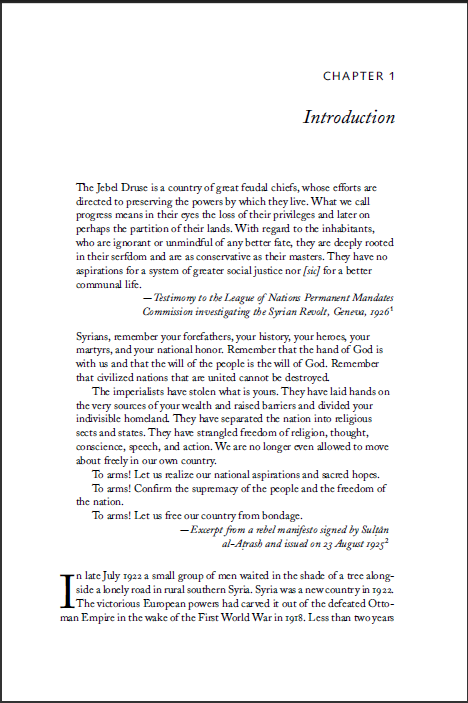
\includegraphics[width=0.95\textwidth]{chapter43.jpg}\par
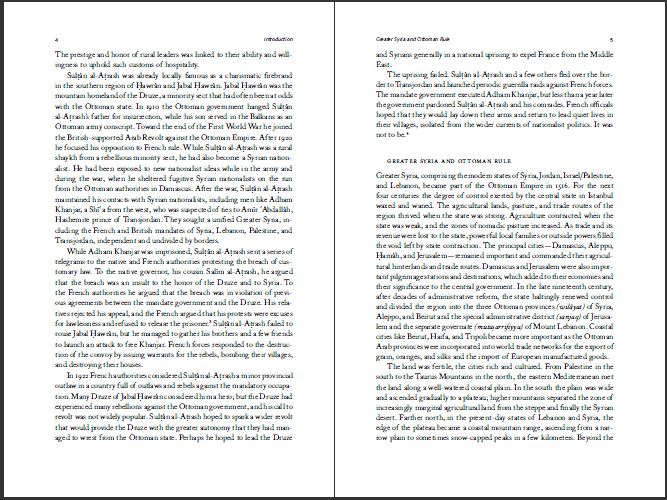
\includegraphics[width=0.95\textwidth]{chapter43a.jpg}
\end{figure}
\everypar{}


\example Naming the template and adding it to the default templates available with your distribution. This template I have named it the \textit{Syrian Revolution} template following the title of the book and as it is
easier to remember than style43. The style43 also exists as an alias. 

\begin{verbatim}
\cxset{syrian revolution/.style={%
 name=CHAPTER,
 number dot=,
 numbering=arabic,
 number font-size=\Large,
 number font-weight=\normalfont,
 number before={},
 number position=rightname,
 chapter color= black!80,
 chapter font-family=\arial,
 chapter font-weight=\normalfont,
 chapter font-size=\Large,
 chapter before=\par\hfill\hfill,
 chapter spaceout=none,
 number after=,
 chapter after=\vskip20pt,
 number color= black!95,
 title font-family=,
 title font-color= black!95,
 title font-weight=\itshape,
 title font-size=\LARGE,
 title font-shape=\itshape,
 title spaceout=none,
 title beforeskip=\hfill,
 epigraph width=0.95\textwidth,
 epigraph font-size=\normalfont,
 author block=false}}

\end{verbatim}














